\section{Production functions}

\begin{frame}{}{}
	\begin{center}
		{\Large Estimating production functions}
	\end{center}
\end{frame}


\begin{frame}{}
	Production function of firm $j$:
	\be
		Q_j = F_j(K_j, L_j)
	\ee
	Most people approximate $F(\cdot)$ with the Cobb-Douglas function
	\be
		Q_j = A_jK_j^{\beta_k}L_j^{\beta_\ell}
	\ee
	The same in logs:
	\be
		q_j = \beta_kk_j + \beta_\ell\ell_j + \ln{A_j}
	\ee
	Is this approximation bad? Not really, see the scatterplot below 
	\begin{center}
		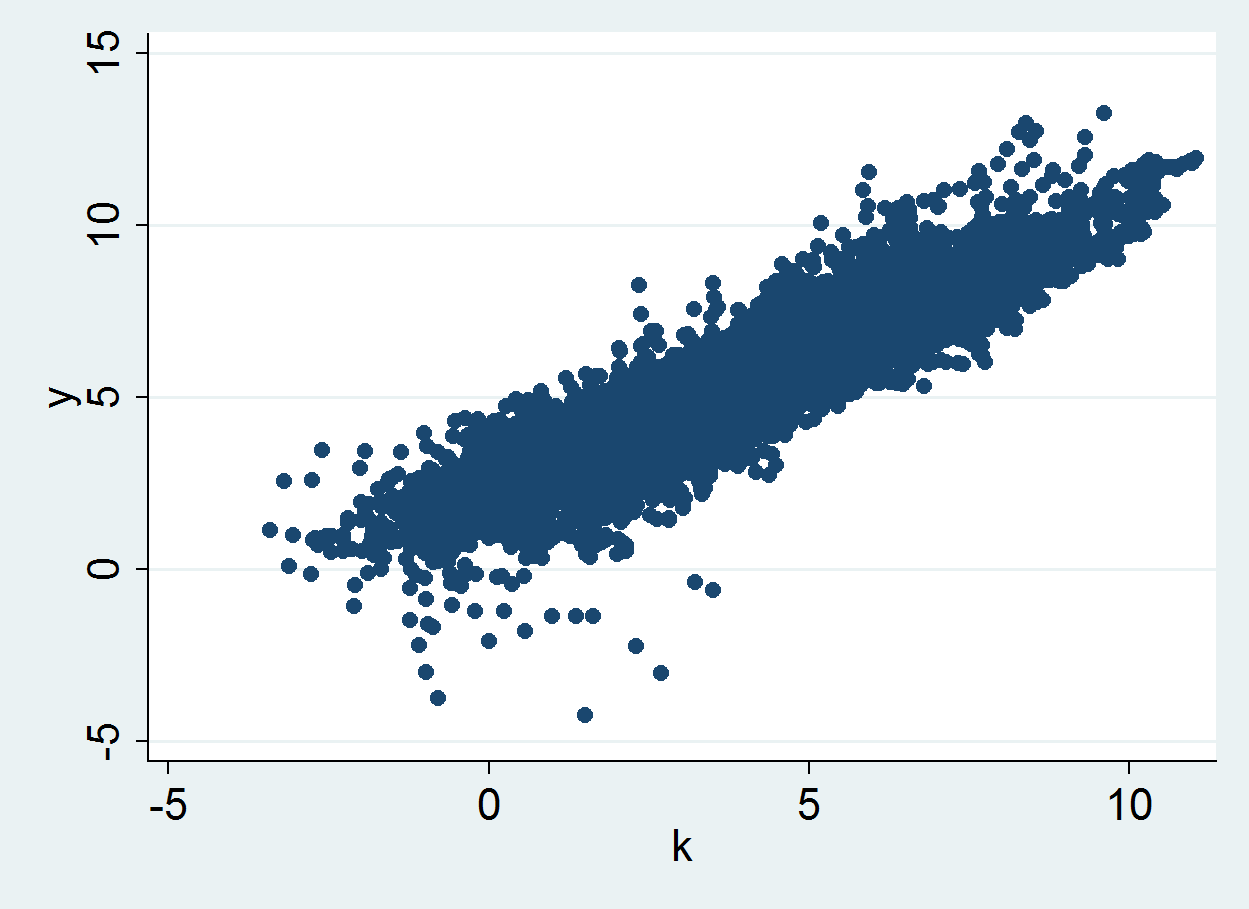
\includegraphics[width=0.4\textwidth]{Figures/yk.png}
		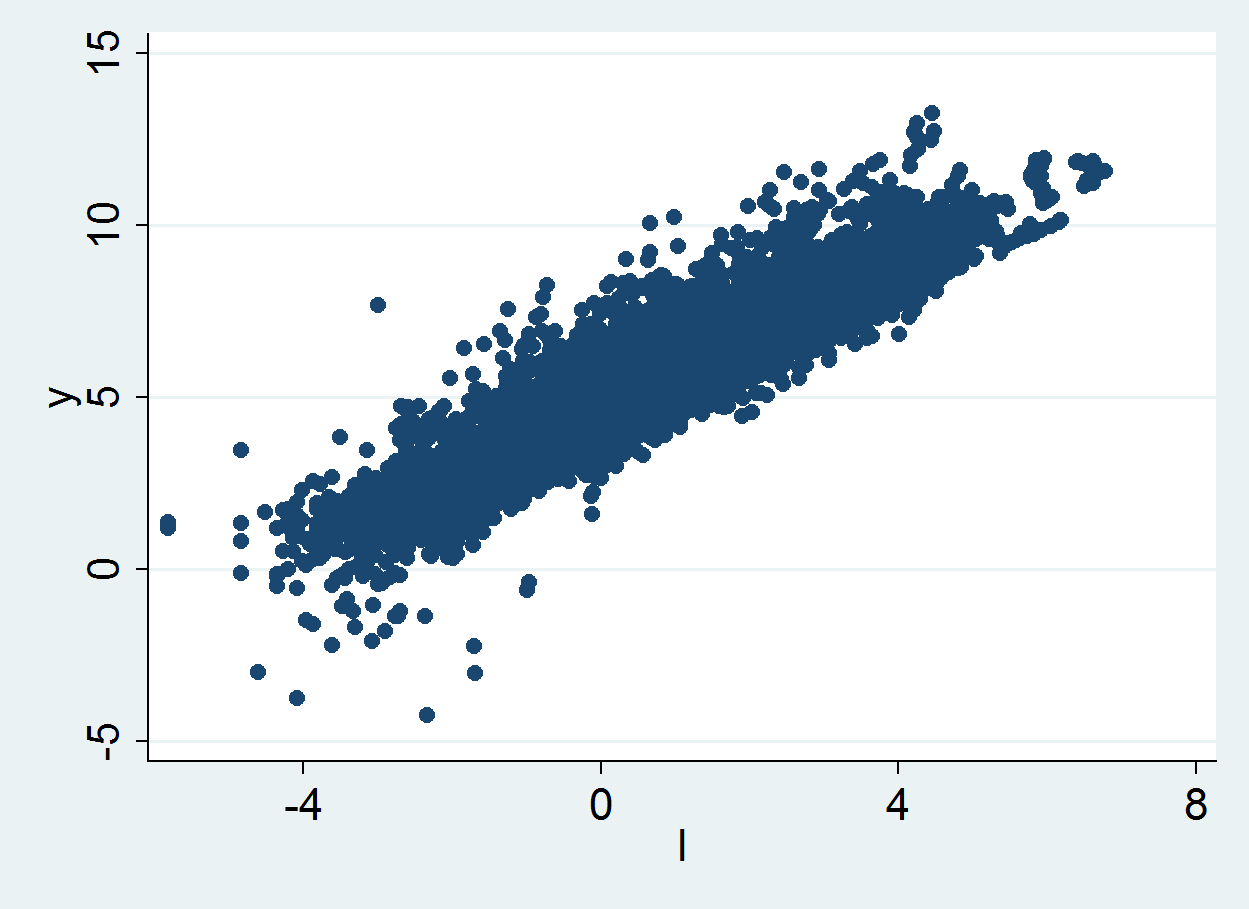
\includegraphics[width=0.4\textwidth]{Figures/yl.png}\\
		\footnotesize(Source: S\&P Compustat firm-level data)
	\end{center}
\end{frame}

\begin{frame}{Applications}
	\bi
		\item{$\beta_k$ and $\beta_\ell$ are informative of the returns to scale. Knowledge of the returns to scale is important for policymakers\\\smallskip
		\textbf{Example:} should we tolerate market concentration? If $\beta_k + \beta_\ell > 1$, then maybe yes, bigger firms are more efficient.}
		
		\item{What drives total factor productivity, $A_j$?\\\smallskip
		
		\textbf{Examples:} 
		\begin{enumerate}
			\item{Endogenous growth theories: industrial activity $\Rightarrow$ learning by doing $\Rightarrow$ knowledge spills over, productivity $\uparrow$: $A_j = f_j(\sum_kQ_k)$. Is this consistent with data?}
			\item{Competition and efficiency: competitive pressure (e.g. trade liberalization) $\Rightarrow$ firms innovate, cut costs, $A_j\uparrow$}
		\end{enumerate}}
		\item{Productive and unproductive firms coexist within the same industry. Sign of restricted competition? Preferential treatment?}
		\item{Aggregate productivity is increasing. What's the mechanism? Existing plants improve? Survival of the fittest? Inputs reallocate to more efficient units?}
	\ei
\end{frame}

\subsection{Rough approximations}
\begin{frame}{Rough approximations}
	Labor productivity = revenue (or value-added) per worker.
	\begin{itemize}
		\item{Easy to compute, low data requirements.}
		\item{But what about other factors? Inefficient allocation of capital (think of SOEs in China or India)?}
	\end{itemize}
	Classic Solow residual:
	\begin{itemize}
		\item{\textbf{Flexible factors}, firms are \textbf{price-takers} in the factor markets:
		\be
			\beta_k = \frac{pQ_j}{rK_j}, \quad \beta_\ell = \frac{pQ_j}{wL_j}
		\ee
		Easy: costs and revenues other than $rK_j$ come from balance sheets. Capital rental costs --- not so easy, but doable.}
		\item{Cons: strong assumptions.}
		\item{Further developments: Erwin Diewert on index numbers.}
	\end{itemize}
\end{frame}


\subsection{OLS Estimator}

\begin{frame}{OLS estimator}
	Data: $q_j, k_j, \ell_j$, for $j=1,\dots,N$.	The econometrician does not observe $A_j$.\\\medskip
	
	Let $\ln{A}_j = \beta_0 + e_j$ so that $E[e_j] = 0$. Then we obtain
	\be
		q_j = \beta_0 + \beta_kk_j + \beta_\ell\ell_j + e_j
	\ee
	A mindless way to estimate this equation is to use OLS:
	\be
		\widehat{\beta} = \left[
		\begin{array}{c}
			\widehat{\beta}_0\\
			\widehat{\beta}_k\\
			\widehat{\beta}_\ell
		\end{array}\right] = \left(\sum_jX_jX_j'\right)^{-1}\sum_jX_jq_j,\quad\text{where }
		X_j = \left[
		\begin{array}{c}
			1\\
			k_j\\
			\ell_j
		\end{array}\right]
	\ee
	This implicitly assumes that $X$ is exogenous, that is, $E[X_je_j]=0$.
\end{frame}

\begin{frame}
	But what is the underlying model that generated the data?	
	\begin{block}{Profit maximization}
		Each firm maximizes its profit, $p_jA_jK_j^{\beta_k}L_j^{\beta_\ell} - w_jL_j - r_jK_j$, given
		\bi
			\item{}input prices, $r_j$ and $w_j$,
			\item{}the level of own productivity, $A_j$, 
			\item{}the price of the final good (normalized to one).
		\ei
		Profit maximization implies
		\begin{equation*}
			\beta_\ell = \frac{p_jQ_j}{w_jL_j}
		\end{equation*}
		or, in logs
		\be
			\ln{\beta_\ell} = q_j + \ln{p_j} - \ell_j - \ln{w_j}.
		\ee
		After substituting  $q_j = \beta_0 + \beta_kk_j + \beta_\ell\ell_j + e_j$ and solving for $\ell_j$,
		\be
			\ell_j = (1-\beta_\ell)^{-1}(\beta_0 + \beta_kk_j + \ln{p_j}- \ln{\beta_\ell}- \ln{w_j} + e_j)
		\ee
		Productivity shock $e_j$ is transmitted to $\ell_j$, \textbf{which violates the exogeneity assumption of OLS}
	\end{block}
\end{frame}

\begin{frame}{}
	Another issue -- endogenous sample selection. The observed data doesn't cover firms after they exit.
	\begin{block}{Models of entry/exit (2nd half of this course)}
		Exiting firms tend to be small and inefficient (low $\ell_j$ and $e_j$).
			
		This makes $\widehat{\beta}$ biased:
		\begin{center}
			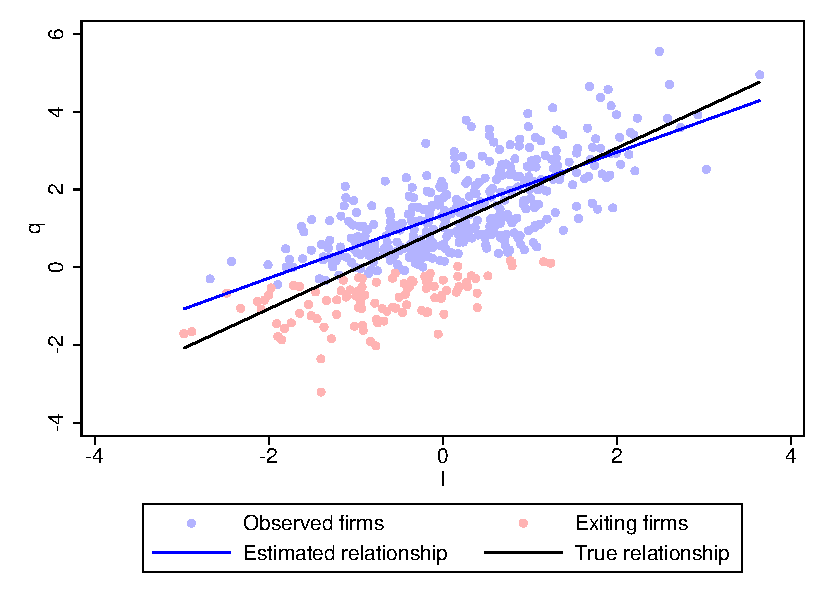
\includegraphics[width = 0.6\textwidth]{Figures/selection_bias.pdf}
		\end{center}
	\end{block}
	\textbf{Verdict:} Avoid using OLS.
\end{frame}

\begin{frame}{IV?}
Why not using IV? We need something that affects the inputs, but does not correlate with unobserved productivity shocks.
\begin{itemize}
	\item{Factor prices? Firm-level data on factor prices rarely available.}
	\item{If available, firm-level variation is likely to reflect quality of inputs. Circumstantial evidence suggests that productivity and input quality are often complementary --- inputs and $e_j$ are correlated.}
	\item{Firms have market power in upstream markets --- factor prices are endogenous.}
	\item{If markets for factors are big, cross-firm variation may be too small to pick up anything ($\sim$ weak instruments).}
\end{itemize}
\end{frame}

\subsection{Fixed effects}

\begin{frame}{The anatomy of error}
	Let's introduce the time dimension so that we can think about the timing of events in our model:
	\be
		q_{jt} = \beta_0 + \beta_kk_{jt} + \beta_\ell\ell_{jt} + e_{jt}
	\ee
	It is helpful to split the residual $e_{jt}$ into two components:
	\be
		e_{jt} = u_{jt} + w_{jt}
	\ee
	Neither $u_{jt}$, nor $w_{jt}$ are observed by the econometrician.
	\bi
		\item{$u_{jt}$ is observed by the firm \emph{before} the firm adjusts $\ell_{jt}$ and $k_{jt}$}
		\item{$u_{jt}$ may include important variables unavailable in data (managerial efficiency, input quality, intangibles, etc.)}
		\item{$w_{jt}$ is unexpected to the firm and is only observed after $\ell_{jt}$ and $k_{jt}$ are set (an earthquake, unusual weather, unexpected demand conditions)}
		\item{$w_{jt}$ may affect the distribution of $u_{jt+1}$ (and hence $(\ell_{jt+1}, k_{jt+1})$), but cannot affect $(\ell_{jt}, k_{jt})$}
	\ei
\end{frame}

\begin{frame}{}
	The problem of endogenous inputs is caused by $u_{jt}$, not by $w_{jt}$:
	\be
		E[X_{jt}e_{jt}] = E[X_{jt}(u_{jt} + w_{jt})] = E[X_{jt}u_{jt}] + E[X_{jt}w_{jt}] = E[X_{jt}u_{jt}] \neq 0
	\ee
	We would like to get rid of $u_{jt}$.
\end{frame}


\begin{frame}{Fixed effects}
	Let's assume that $u_{jt}$ has, in turn, two components: $u_{jt} = v_j + \delta_t$. That is
	\bi
		\item{If $u_{jt}$ represents managerial talent, bad managers can't really improve}
		\item{If $u_{jt}$ captures the variation in input quality, this quality changes at the same rate for all firms}
		\item{Etc.}
	\ei
	I.e. whatever is captured by $u_{jt}$, it is either constant or changes at the same rate for everyone.
\end{frame}


\begin{frame}{}
	Main equation:
	\begin{align*}
		q_{jt} &= \beta_0 + \beta_kk_{jt} + \beta_\ell\ell_{jt} + v_j + \delta_t + w_{jt}\\
		&= X_{jt}\beta + v_j + w_{jt}
	\end{align*}
	where $X_{jt}$ includes $k_{jt}$, $\ell_{jt}$ and year dummies. After subtracting the means:
	\be
		q_{jt} - \overline{q}_{j} = (X_{jt} - \overline{X}_{j})\beta + (w_{jt} - \overline{w}_j)
	\ee
	There is no $u_{jt}$ anymore! The error term, $(w_{jt} - \overline{w}_j)$,
	\bi
		\item{does not affect the firm's choice of inputs}
		\item{does not affect the firm's entry/exit decisions}
	\ei 
	This equation can be safely estimated by OLS.
\end{frame}

\begin{frame}{}
	Fixed effects estimator comes with an implicit assumption -- strict exogeneity:
	\be
		E[X_{jt}w_{js}] = 0 \text{ for any $t$ and $s$}
	\ee
	Strict exogeneity ensures that
	\be
		E[(X_{jt} - \overline{X}_{j})(w_{jt} - \overline{w}_j)] = 0
	\ee
	But this can be relaxed by modifying the estimator. Take the differences instead:
	\be
		\Delta{}q_{jt} = q_{jt} - q_{jt-1} = \Delta{}X_{jt}\beta + \Delta{}w_{jt}
	\ee
	Then, use the IV estimator instrumenting $\Delta{}X_{jt}$ with $X_{jt-1}$. This estimator relies on a much weaker assumption:
	\be
		E[(w_{jt} - w_{jt-1})X_{jt-1}] = E[w_{jt}X_{jt-1}] = 0
	\ee
	Intuitively, this should be okay: at the time when $X_{jt-1}$ is realized, $w_{it}$ is unknown and unexpected.
\end{frame}

\begin{frame}{Problems: returns to scale too low}\
	\begin{center}
	\begin{tabular}{|c|cc|}\hline
		Estimator & OLS 	& Fixed effects \\\hline
		Labor 	& 0.693	& 0.629 \\
				& (0.019)	& (0.026) \\
		Capital	& 0.304	&  0.150 \\
				& (0.018)	&  (0.026) \\\hline
	\end{tabular}\\
	{\footnotesize{}Source: Olley \& Pakes (1996)}
	\end{center}
	\bi
		\item{This is systematic; FE estimates suggest decreasing returns to scale in numerous datasets}
		\item{Using balanced panel vs full panel often has big impact on FE. Shouldn't happen if FE addresses endogeneity.}
		\item{General consensus: low returns to scale are caused by some econometric bias}
		\item{Nobody is certain what is the exact reason}
	\ei
		\textbf{Verdict:} FE estimator is okay in a preliminary analysis. Otherwise, people tend not to take the FE estimates too seriously.
\end{frame}